%!TEX root = ../../thesis.tex

\part{Applications: Viruses and Bacteria}
\label{part:application_microorganism}

% Bacteriophage Mosaicism
% Primarily based on the dataset in Lima-Mendez
% Just basic results + Ayasdi figure
%!TEX root = ../../thesis.tex
\chapter{Phage Mosaicism}
\label{ch:phage}

\section{Introduction}
\label{phage:introduction}

Phages are microbial viruses which can infect bacteria, archaea, or single-celled eukaryotes.
By some measures, they are the most abundant and diverse class of organism on the planet.
It is estimated that there are $10^{31}$ extant bacteriophages \cite{Rohwer:2014vz}.\footnote{The estimate can be arrived at two independent ways: by assuming a total bacterial population size of $10^{30}$, and approximately ten phages per bacteria; or by the observation of a phage density of $10^{6}$ to $10^{7}$ per mL of seawater.}
The phage population completely turns over every few days -- an estimated infection rate of $10^{23}$ per second \cite{Suttle:2007cj}.

Phages play an essential role in natural ecosystems by regulating bacterial populations.
Steps have been taken towards harnessing this ability for productive use -- the FDA has approved several bacteriophage products designed to kill harmful bacteria in dairy and meat products \cite{Bren:2007wn}.
Also promising are potential phage therapies for treating pathogenic bacterial infections, although research in this direction is controversial \cite{Keen:2012du}.

Phages are classified based on lifestyle: virulent phages have a lytic life cycle and will infect a host, multiply, and exit the cell via lysis, killing the host organism; temperate phages have a lysogenic life cycle and can remain within the host in a latent state, without disrupting host cellular function.
Phages can have a nucleic acid composition that is either double-stranded DNA (dsDNA), single-stranded DNA (ssDNA), double-stranded RNA (dsRNA), or single-stranded RNA (ssRNA).
Of these, dsDNA is by far the most common.
The typical phage genome length is on the order of $10^{5}$ bases, but can range from $10^{3}$ to $10^{6}$ bases.

Because there is no conserved gene across all phage populations, there is no accepted way of constructing a molecular phage taxonomy.
The current bacteriophage taxonomy is compiled by the International Committee on Taxonomy of Viruses (ICTV) and is based on virus morphology, host range, lifestyle, and nucleic acid composition \cite{ICTV:2012}.
Table~\ref{phage:table:families} presents an overview of phage families as defined by the ICTV.
There are two assigned orders and eighteen recognized families.
Fourteen families have dsDNA, two families have ssDNA, and two families have an RNA genome.

% phage:table:families
\begin{table}[t]
    \caption{Phage families defined by the ICTV}
    \centering
    \scriptsize
    \begin{tabularx}{\textwidth}{lXlX}
    \toprule
    Order & Family & Morphology & Nucleic acid \\
    \midrule
    \multirow{3}{*}{\emph{Caudovirales}} & \emph{Myoviridae}   & Nonenveloped, contractile tail           & linear dsDNA \\
                                         & \emph{Siphoviridae} & Nonenveloped, noncontractile tail (long) & linear dsDNA \\
                                         & \emph{Podoviridae}  & Nonenveloped, noncontractile tail (short) & linear dsDNA \\
    \midrule
    \multirow{2}{*}{\emph{Ligamenvirales}} & \emph{Lipothrixviridae} & Enveloped, rod-shaped    & linear dsDNA \\
                                           & \emph{Rudiviridae}      & Nonenveloped, rod-shaped & linear dsDNA \\
    \midrule
    \multirow{13}{*}{Unassigned} & \emph{Ampullaviridae} & Enveloped, bottle-shaped   & linear dsDNA\\
                                 & \emph{Bicaudaviridae} & Nonenveloped, lemon-shaped & circular dsDNA \\
                                 & \emph{Clavaviridae}   & Nonenveloped, rod-shaped   & circular dsDNA \\
                                 & \emph{Corticoviridae} & Nonenveloped, isometric    & circular dsDNA \\
                                 & \emph{Cystoviridae}   & Enveloped, spherical       & segmented dsRNA \\
                                 & \emph{Fuselloviridae} & Nonenveloped, lemon-shaped & circular dsDNA \\
                                 & \emph{Globuloviridae} & Enveloped, isometric       & linear dsDNA \\
                                 & \emph{Guttaviridae}   & Nonenveloped, ovoid        & circular dsDNA \\
                                 & \emph{Inoviridae}     & Nonenveloped, filamentous  & circular ssDNA \\
                                 & \emph{Leviviridae}    & Nonenveloped, isometric    & linear ssRNA \\
                                 & \emph{Microviridae}   & Nonenveloped, isometric    & circular ssDNA \\
                                 & \emph{Plasmaviridae}  & Enveloped, pleomorph       & circular dsDNA \\
                                 & \emph{Tectiviridae}   & Nonenveloped, isometric    & linear dsDNA \\
    \bottomrule
    \end{tabularx}
    \label{phage:table:families}
\end{table}

Phages have been shown to be subject to high rates of reticulate genomic exchange \cite{Westmoreland:1969dd}.
The phage genome was thought to be a mosaic, composed of distinct modules that can be freely exchanged within a population.
Increased genomic data has confirmed this mosaic structure and raised questions about the applicability and interpretation of the ICTV taxonomy.
Based solely on morphology, the ICTV taxonomy has been shown to be inconsistent with the genomic data, as the following example from Lawrence \emph{et al.} shows \cite{Lawrence:2002eg}.
In Figure~\ref{phage:fig:inconsistency} we show three different bacteriophage species: Enterobacteria phage HK97, Mycobacterium phage L5, and Enterobacteria phage P22.
HK97 is a Siphoviridae infecting \emph{E. coli}.
L5 is a Siphoviridae infecting \emph{M. smegmatis}.
P22 is a Podoviridae infecting \emph{S. enterica}.
HK97 and L5 belong to the Siphoviridae family comprised of long tail noncontractile phages.
P22 belongs to the Podoviridae family comprised of short tail phages.
Visually, it appears that HK97 and L5 should indeed be classified as distinct from P22.
However, genomic analysis reveals that HK97 and L5 share no gene content, and, despite appearances to the contrary, HK97 and P22 share 20\% gene content.
This example demonstrates that morphology and host range alone are not sufficient in representing phage relationships.

\begin{figure}
\centering
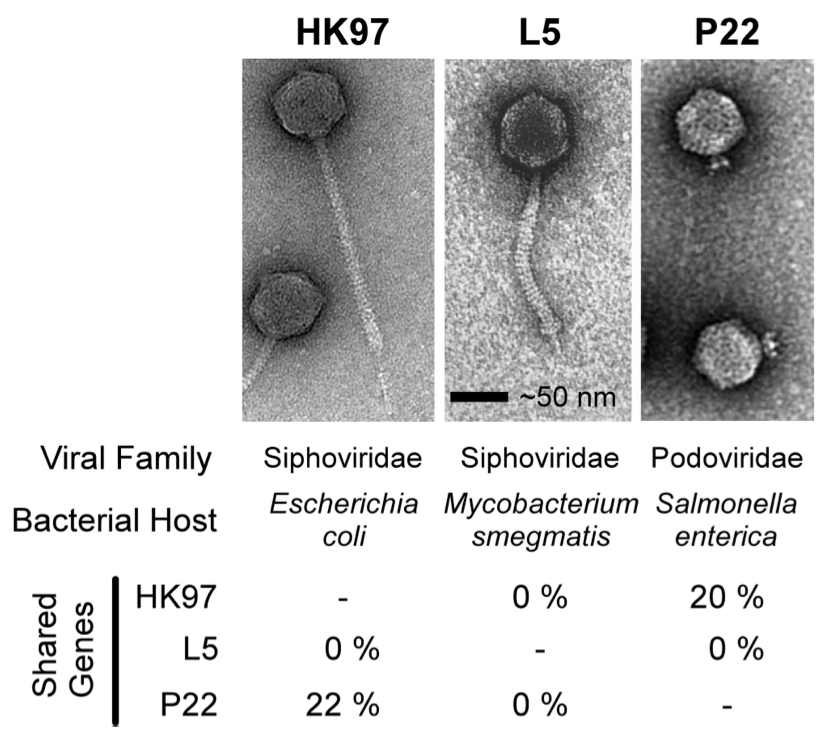
\includegraphics[width=.5\linewidth]{./fig/phage/LAWRENCE_phage_comparative.png}
\caption[Inconsistency of morphological classifications in bacteriophage]{Inconsistency of morphological classifications in bacteriophage. HK97 and L5 are classified in the Siphoviridae family of long tail non-contractile phages, despite sharing no gene content. P22, a short-tail phage in the Podoviridae family, while morphologically dissimilar, shares 20\% gene content with HK97. Figure adapted from \parencite{Lawrence:2002eg}.}
\label{phage:fig:inconsistency}
\end{figure}

Alternative representations of phage relationships have been proposed based on whole genome analysis.
For example, Rohwer and Edwards constructed a phage phylogenetic tree using differences in phage proteomes \cite{Rohwer:2002uo}.
Proux \emph{et al.} proposed a phylogenetic representation based on comparative analysis of head and tail sequences \cite{Proux:2002gj}.
However, these models still make the assumption of tree-like relationships, which will not be appropriate for representing highly mosaic molecular relationships.

In this chapter, we use approaches from topological data analysis to identify, measure, and represent reticulate evolution in a population of phage sequences.
This work is primarily based on data collected by Lima-Mendez \emph{et al.} \cite{LimaMendez:2008ki}.
First, we use persistent homology to characterize reticulation in phage genomes.
We find $H_0$ is largely inconsistent with existing phage taxonomies, and interpret $H_1$ as evidence for reticulate genetic exchange due to shared ecology and host range.
Second, we visualize phage molecular relationships using Mapper, identifying clusters of phages with common gene content and host range.
The Mapper network suggests an alternate way of representing phage relationships.

\section{Data}

We use data initially collected an analyzed in \cite{LimaMendez:2008ki}.
The initial data set consists of a collection of 306 sequenced bacteriophage genomes.
We show summary information about the data in Figure~\ref{phage:fig:phage_data_plot}.
Of the 306 genomes, 246 consist of dsDNA, 36 ssDNA, 12 dsRNA, and 8 ssRNA.
Four have unclassified nucleic acid material.
With respect to lifestyle, 146 are temperate and 72 are virulent.
Actinoplanes phage phiAsp2 is the single pseudotemperate phage, which means it largely maintains a temperate lifestyle but can occasionally enter a virulent state.
For 87 phages the lifestyle is unknown.
Taxonomically, the vast majority belong to order Caudovirales (221), which comprises Siphoviridae (117), Myoviridae (47), and Podoviridae (54). 
Order Ligamenviralies (4) comprises Lipothrixviriae (2) and Rudiviridae (2).
Unassigned families include Inoviridae (22), Cystoviridae (12), Gokushoviridae (8), and Microviridae (6).

\begin{figure}
\centering
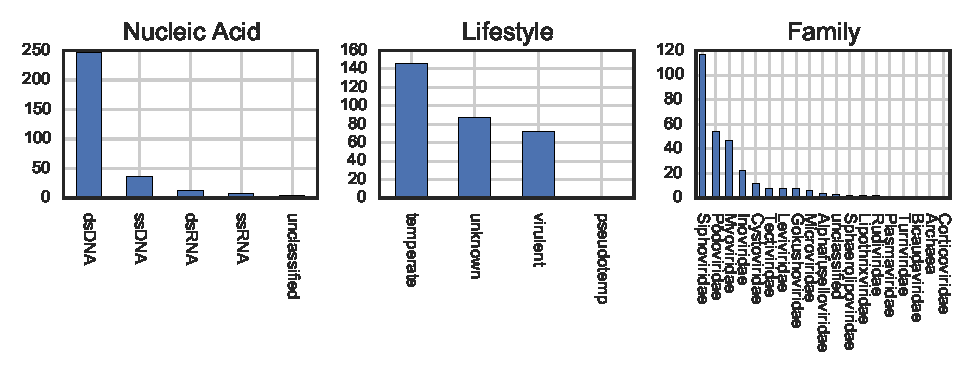
\includegraphics[]{./fig/phage/phage_data_plots.pdf}
\caption[Summary annotations of 306 bacteriophage strains used in this study]{Summary annotations of phage data used in this analysis. 306 bacteriophage genomes were included, as originally collected in \cite{LimaMendez:2008ki}. Here we show various annotations for the phage, including nucleic acid type, lifestyle, and taxonomic family (as defined by the ICTV). For some phage strains this data is unknown.}
\label{phage:fig:phage_data_plot}
\end{figure}

Each of the 306 bacteriophage genomes has been sequenced and annotated.\footnote{The annotation step assigns genes to subsequences of the genome. For well-characterized species this is facilitated by a reference genome. For less well-characterized species this can require the use of heuristic gene-finding algorithms.}
This step resulted in 19,537 unique bacteriophage phage genes.
In the original study \cite{LimaMendez:2008ki}, these genes were then clustered into 8,576 protein families using BlastP, which analyzes pairwise similarity of proteins \cite{Altschul:1997a}.
Protein families share homology, which implies some degree of shared evolutionary ancestry.
Phages can then be represented as phyletic profiles in a protein family-space, indicating the presence or absence of a particular protein family.
In this case, the phyletic matrix $P$ is a $306\times19537$ binary matrix.

\section{Measuring Phage Mosaicism with Persistent Homology}
\label{phage:ph}

We apply persistent homology to the phyletic profiles in order to quantify reticulation in the bacteriphage data.
Because we have transformed from sequence space into phyletic profiles, we do not invoke a specific evolutionary model.
However, the fundamental theorem that non-trivial homology implies reticulation will still hold.
First, we construct an appropriate metric space.
Following \cite{LimaMendez:2008ki}, we use a hypergeometric model as follows.
For two phages $A$ and $B$, let $a$ be the number of protein families in phage $A$, $b$ be the number of protein families in phage $B$, and $c$ be the number of protein families in common.
Let $n$ be the total number of protein families.
Then we can compute the p-value that the number of shared protein families $c$ is significant as
\begin{equation}
P_{AB} = \sum_{i=c}^{\min(a,b)} \frac{\binom{a}{i}\binom{n-a}{b-i}}{\binom{n}{b}}.
\end{equation}
To convert the p-values into a distance we take the log transform with small added noise,
\begin{equation}
d_{AB} = \log_{10}(P_{AB} + 10^{-10}) + 10.
\end{equation}
This yields a distance matrix $D$ with distances scaled between $0$ and $10$.
While this space does not explicitly reflect evolutionary divergence at a molecular level, it may be realistic at the protein level at which more complex types of genome evolution will have occurred.

We now compute the persistent homology of $D$.
The barcode diagram is shown in Figure~\ref{phage:fig:barcode}.
The $H_0$ information represents hierarchical clustering and can be identically represented as a dendrogram.
We show the dendrogram, restricting only to strains of order Caudovirales, in Figure~\ref{phage:fig:caudosubset_dendrogram}.
The strains are labeled by their taxonomic family: red for Myoviridae, blue for Siphoviridae, and green for Podoviridae.
We can immediately see that the assigned taxonomic families are not consistent with the clustering based on protein information.
However, there does appear to be some structure in which the taxonomic label is consistent within clusters of strains.
Returning to the barcode diagram, we see substantial nontrivial homology in $H_1$ across all scales.
This confirms the presence of mosaic exchange expected in phage genomes.
% Cycles in $H_1$ can be mapped to specific reticulation patterns. (include???)

\begin{figure}
\centering
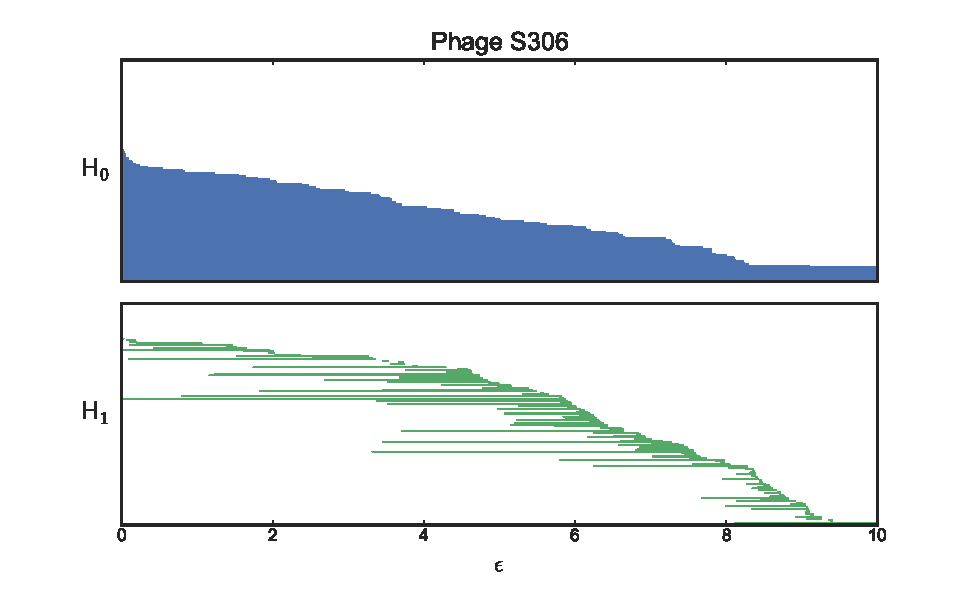
\includegraphics[]{./fig/phage/phage_s306_barcode.pdf}
\caption[Bacteriophage Barcode Diagram]{Bacteriophage Barcode Diagram using the S306 dataset.}
\label{phage:fig:barcode}
\end{figure}

\begin{figure}
\centering
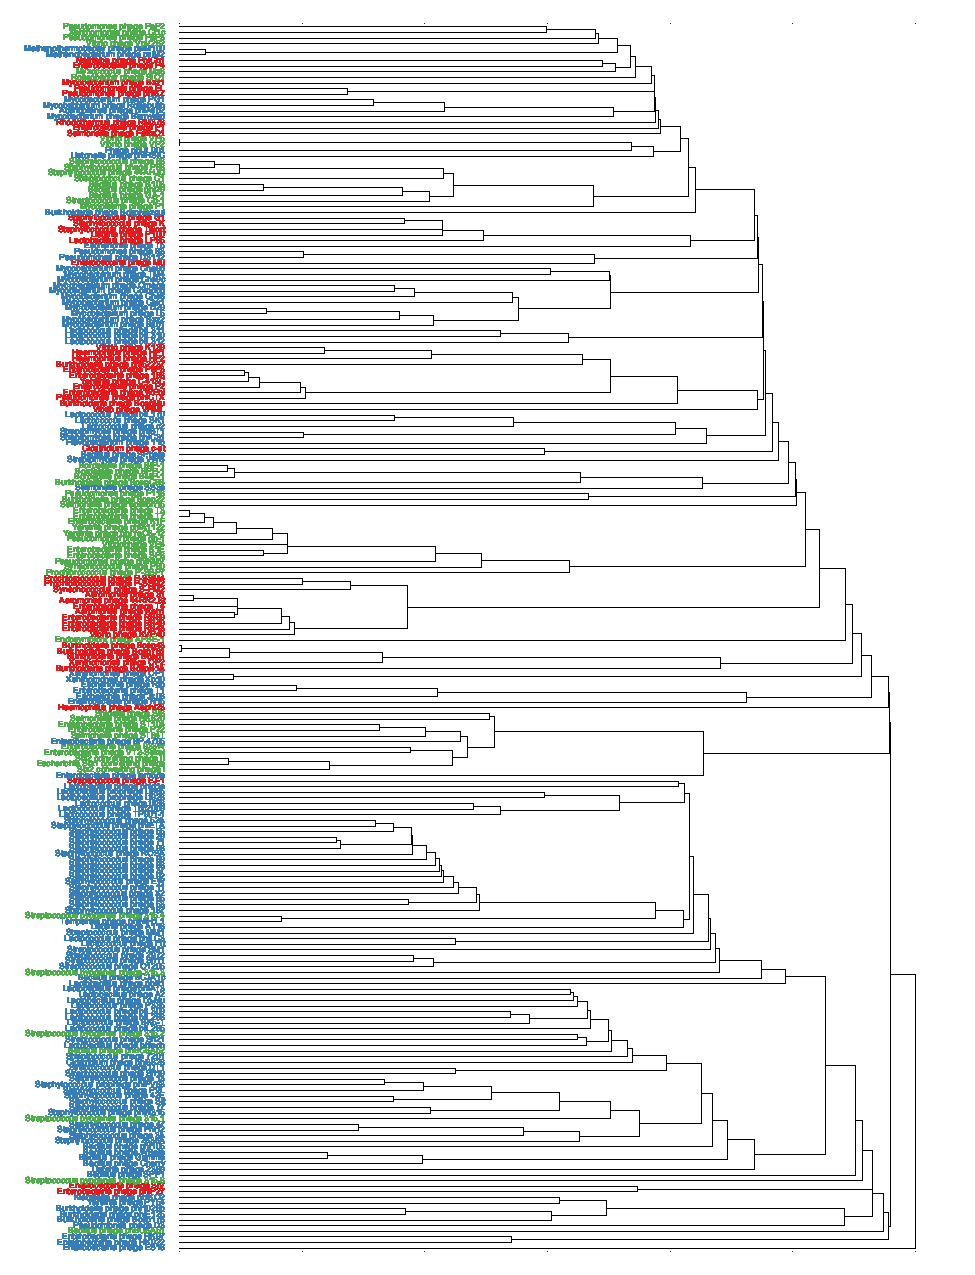
\includegraphics[]{fig/phage/phage_s306_caudosubset_dendrogram.pdf}
\caption[Caudovirales $H_0$ dendrogram]{The dendrogram constructed from the $H_0$, restricted to bacteriophages of order Caudovirales. Myoviridae in red, Siphoviridae in blue, and Podoviridae in green. The family classifications are inconsistent with the hierarchical clustering.}
\label{phage:fig:caudosubset_dendrogram}
\end{figure}

Focusing on order Caudovirales, for which the most data was present.
We separately computed persistent homology for each of the three families.
The barcode diagrams are shown in Figure~\ref{phage:fig:caudovirales_barcodes}.
%% TODO: make a comment?

\begin{figure}
\centering
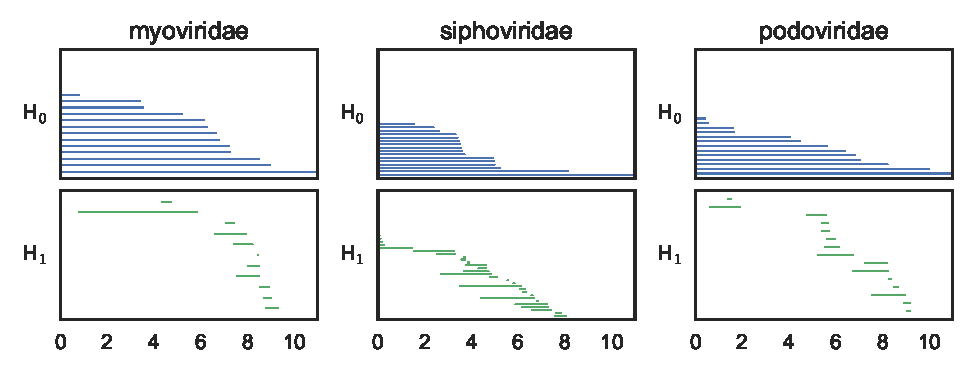
\includegraphics[]{{./fig/phage/phage_s306_caudovirales_barcodes}.pdf}
\caption[Caudovirales Barcode Diagrams]{Barcode Diagrams for Families of Order Caudovirales, including Siphoviridae, Myoviridae, and Podoviridae.}
\label{phage:fig:caudovirales_barcodes}
\end{figure}

\section{Representing Phage Relationships with Mapper}
\label{phage:mapper}

We used Ayasdi Mapper to construct a network representation of the phage phyletic profiles.
The network was constructed using a Hamming metric on the binary phyletic matrix and a 2D filter function.
The first filter was Metric PCA coordinate 1 with a resolution of 20 and a gain of 3.\footnote{The parameter settings are in arbitrary units and tuned by hand to produce the most visually useful graph.}
The second filter was metric PCA coordinate 2 with a resolution of 20 and a gain of 3.
The equalize setting was used for both filter functions, which ensures that in the filtered space each bin has approximately the same number of points.
This resulted in a network consisting of 201 nodes from the original 306 rows.
The basic structure of the network is shown in Figure~\ref{phage:fig:phage_mapper_network}, where node color corresponds to the number of rows contained in the node.
The network consists of one large connected component, two smaller connected components, and 21 singly connected nodes.

\begin{figure}
\centering
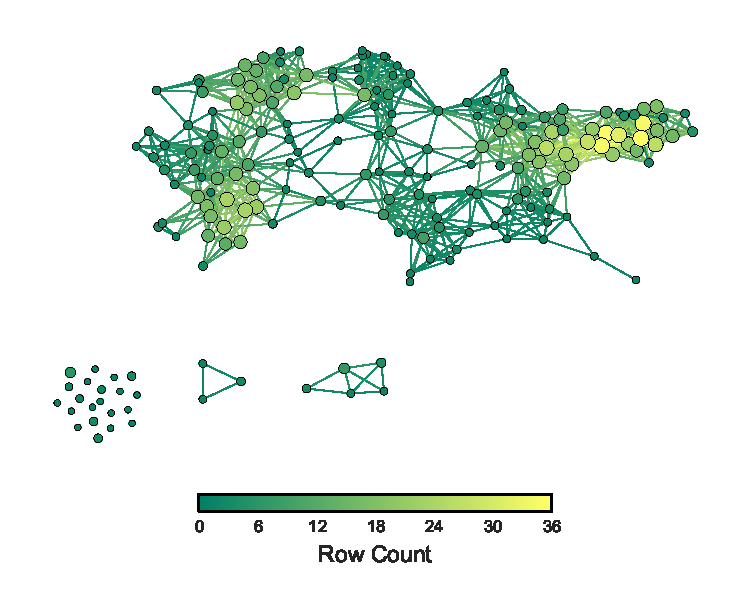
\includegraphics[]{{fig/phage/phage.s306.mapper_network}.pdf}
\caption[Phage Mapper Network]{Phage Mapper Network}
\label{phage:fig:phage_mapper_network}
\end{figure}

We first examined how well existing taxonomic classifications mapped onto this representation.
If the taxonomy is accurate, we would expect to see a tight clustering of particular orders, with minimal overlap
We show the representation of the three families of order Caudovirales in Figure~\ref{phage:fig:s306_caudovirales_networks}.
Each node is colored by the proportion of rows in that particular family.
We can immediately see that each family is widely dispersed across the network.

How strongly a particular classification is reflected by a network can be quantitatively measured using a modularity score \cite{Newman:2006iq}.
Modularity was originally devised for identifying community structure in networks.
Intuitively, more tightly localized network divisions will have a higher modularity, while dispersed divisions will have a lower modularity.
The basic definition for a two-class division is
\begin{equation}
Q = \frac{1}{4m}\sum_{ij}\left( A_{ij} - \frac{k_{i}k_{j}}{2m} \right)(s_{i}s_{j}+1)
\end{equation}
where $m$ is the total number of edges in the network, $A$ is the adjacency matrix of the network, $k_i$ is the degree of node $i$, and $s_{i}=\pm1$ is the class membership of node $i$.
We adopt a slightly modified 

\begin{figure}
\centering
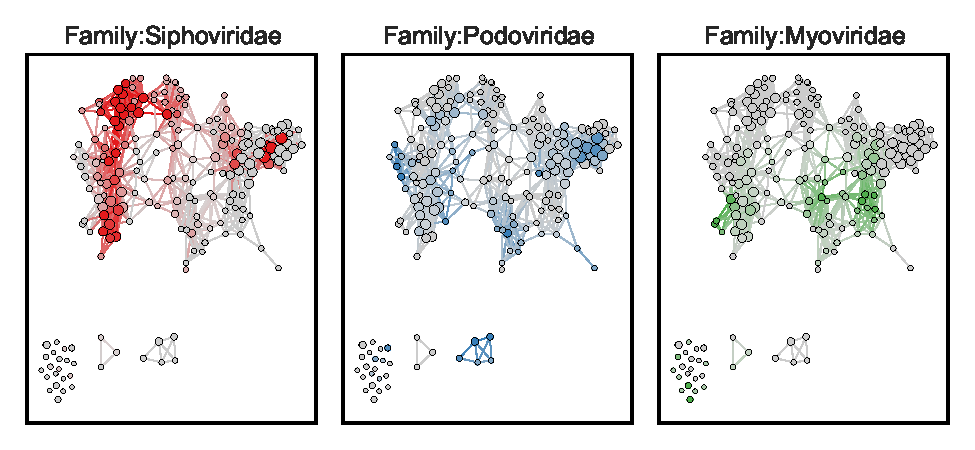
\includegraphics[]{{fig/phage/phage.s306.caudovirales_networks}.pdf}
\caption[Caudovirales Family Networks]{Caudovirales Family Networks}
\label{phage:fig:s306_caudovirales_networks}
\end{figure}

Second, we examined how well host correlated with network structure.
We show this for the top six hosts represented in our dataset in Figure~\ref{phage:fig:s306_host_networks}.
We see that while Enterobacteria has several pockets of representation within the network, phages are indeed more strongly clustered by host than by taxonomy.
This is consist with existing evidence that phages of similar host range have a common environment for horizontal gene transfer.

\begin{figure}
\centering
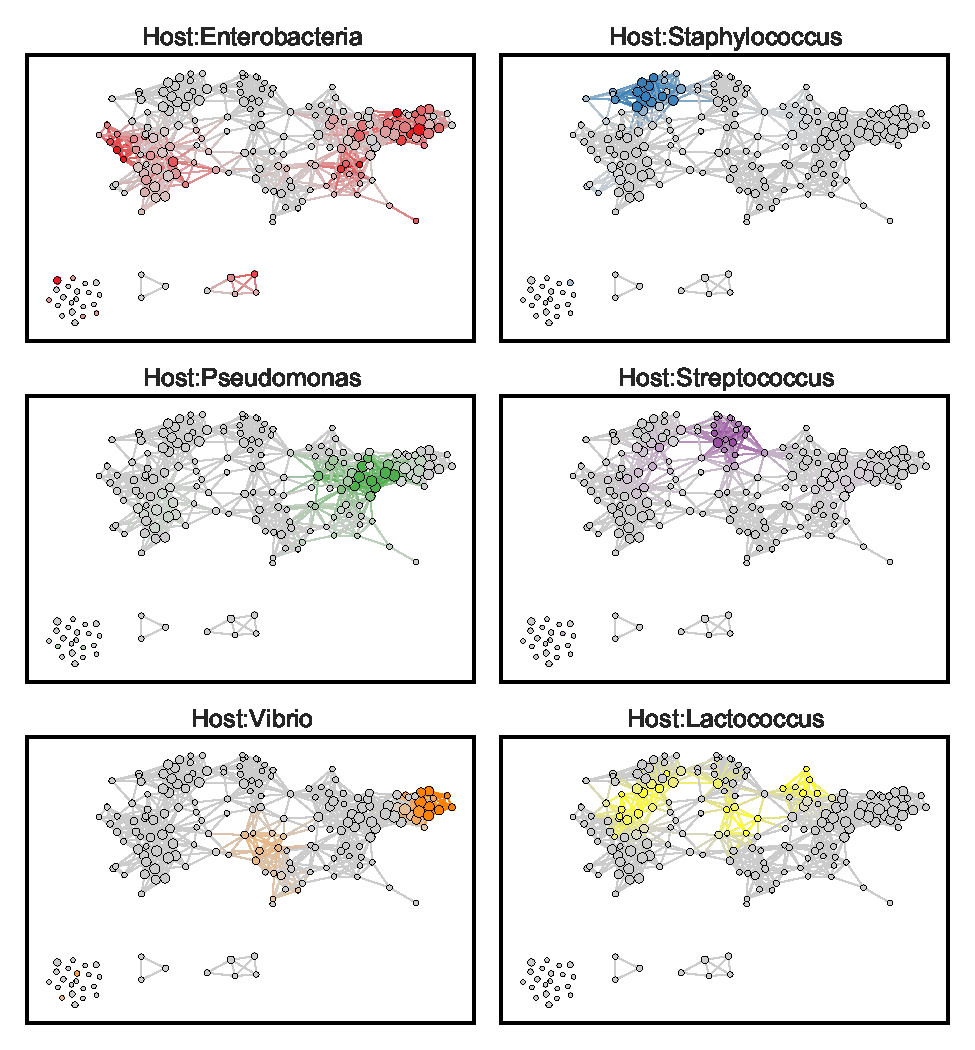
\includegraphics[]{{fig/phage/phage.s306.host_networks}.pdf}
\caption[Phage Host Networks]{Phage Host Network.}
\label{phage:fig:s306_host_networks}
\end{figure}

Finally, we clustered the network using the MCL graph clustering algorithm \cite{Enright:2002ep}, as implemented in the Python MCLMarkovCluster package \cite{Lami:2014}.
The MCL algorithm takes two input parameters which control the coarseness of the clustering: an expansion factor $e$ and an inflation factor $i$.
We set $e=5$ and $i=5$.
Ignoring the singleton nodes, this resulted in eleven clusters, as shown in Figure~\ref{phage:fig:s306_mcl_clustered_network}.
For each cluster, we used a hypergeometric test to identify particular protein families that were over- or under-represented in each cluster.
Correcting for multiple testing ($p=8578$).
The protein families that passed this threshold are shown in Table~\ref{phage:table:cluster_functions}.

\begin{figure}
\centering
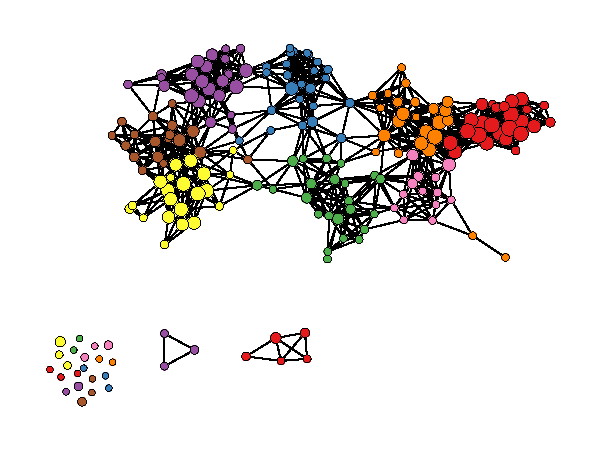
\includegraphics[]{{fig/phage/phage.s306.mcl_clustered_network}.pdf}
\caption[Phage Network with MCL Clustering]{Phage Network with MCL Clustering}
\label{phage:fig:s306_mcl_clustered_network}
\end{figure}

% phage function table.
\begin{sidewaystable}
    \caption{Phage cluster annotations -- protein family functions}
    \tiny

    % define tables
    \begin{lrbox}{\leftbox}
            \begin{tabular}[t]{llll}
            \toprule
            Cluster & Protein Family & p-value & Function \\
            \midrule
            \multirow{1}{*}{Cluster 1} & pf\_0001 & 6.17e-25 & tail tape measure protein \\ 
                                        & pf\_0002 & 6.81e-21 & transcriptional repressor \\ 
                                        & pf\_0003 & 2.69e-16 & tyrosine based integrase \\ 
                                        & pf\_0004 & 9.08e-12 & DNA binding protein \\ 
                                        & pf\_0008 & 7.37e-10 & unknown \\ 
                                        & pf\_0010 & 2.36e-08 & terminase large subunit \\ 
                                        & pf\_0006 & 2.87e-08 & NA \\ 
                                        & pf\_0164 & 5.57e-08 & NA \\ 
                                        & pf\_0012 & 1.74e-07 & DNA replication inititation protein \\ 
                                        & pf\_0015 & 2.42e-07 & scaffolding protein \\ 
                                        & pf\_0187 & 2.70e-07 & NA \\ 
                                        & pf\_0217 & 2.70e-07 & NA \\ 
                                        & pf\_0013 & 3.35e-07 & NA \\ 
                                        & pf\_0017 & 4.63e-07 & portal protein \\ 
                                        & pf\_0007 & 8.84e-07 & endolysin \\ 
            \midrule
            \multirow{1}{*}{Cluster 2} & pf\_0131 & 9.38e-13 & NA \\ 
                                        & pf\_0279 & 2.33e-09 & NA \\ 
                                        & pf\_0109 & 1.02e-08 & NA \\ 
                                        & pf\_0434 & 4.38e-08 & NA \\ 
                                        & pf\_0435 & 4.38e-08 & NA \\ 
                                        & pf\_0436 & 4.38e-08 & NA \\ 
                                        & pf\_0010 & 1.84e-07 & terminase large subunit \\ 
                                        & pf\_0029 & 2.02e-07 & major head protein \\ 
                                        & pf\_0009 & 2.54e-07 & NA \\ 
                                        & pf\_0093 & 4.61e-07 & NA \\ 
                                        & pf\_0512 & 5.47e-07 & NA \\ 
                                        & pf\_0017 & 7.12e-07 & portal protein \\ 
            \midrule
            Cluster 3 & & & \\
            \midrule
            \multirow{1}{*}{Cluster 4} & pf\_0049 & 3.44e-24 & unknown \\ 
                                        & pf\_0043 & 3.44e-24 & unknown \\ 
                                        & pf\_0053 & 3.86e-23 & unknown \\ 
                                        & pf\_0052 & 3.86e-23 & unknown \\ 
                                        & pf\_0007 & 6.19e-22 & endolysin \\ 
                                        & pf\_0058 & 4.39e-21 & unknown \\ 
                                        & pf\_0060 & 4.39e-21 & unknown \\ 
                                        & pf\_0061 & 4.39e-21 & unknown \\ 
                                        & pf\_0002 & 2.23e-20 & transcriptional repressor \\ 
                                        & pf\_0067 & 4.46e-20 & unknown \\ 
                                        & pf\_0063 & 4.46e-20 & unknown \\ 
                                        & pf\_0012 & 1.12e-19 & DNA replication inititation protein \\ 
                                        & pf\_0018 & 2.04e-19 & tail protein \\ 
                                        & pf\_0072 & 4.38e-19 & unknown \\ 
                                        & pf\_0004 & 1.82e-18 & DNA binding protein \\ 
                                        & pf\_0020 & 5.91e-18 & unknown \\ 
                                        & pf\_0087 & 3.86e-17 & unknown \\ 
                                        & pf\_0042 & 5.24e-17 & unknown \\ 
                                        & pf\_0001 & 1.54e-16 & tail tape measure protein \\ 
                                        & pf\_0092 & 3.48e-16 & unknown \\ 
            \midrule
            \end{tabular}
    \end{lrbox}
    \begin{lrbox}{\rightbox}
            \begin{tabular}[t]{llll}
            \toprule
            Cluster & Protein Family & p-value & Function \\
            \midrule
            \multirow{1}{*}{Cluster 5} & pf\_0008 & 7.45e-07 & unknown \\ 
            \midrule
            \multirow{1}{*}{Cluster 6} & pf\_0006 & 2.17e-18 & NA \\ 
                                        & pf\_0057 & 8.74e-10 & unknown \\ 
                                        & pf\_0142 & 3.84e-09 & unknown \\ 
                                        & pf\_0082 & 1.79e-08 & lysis protein \\ 
                                        & pf\_0165 & 2.09e-08 & prohead \\ 
                                        & pf\_0188 & 1.12e-07 & minor tail protein \\ 
                                        & pf\_0190 & 1.12e-07 & tail \\ 
                                        & pf\_0189 & 1.12e-07 & minor tail protein \\ 
                                        & pf\_0204 & 5.81e-07 & unknown \\ 
            \midrule
            \multirow{1}{*}{Cluster 7} & pf\_0002 & 8.92e-11 & transcriptional repressor \\ 
                                        & pf\_0121 & 2.46e-09 & transcription factor  \\ 
                                        & pf\_0016 & 3.36e-08 & unknown \\ 
                                        & pf\_0122 & 6.52e-08 & unknown \\ 
                                        & pf\_0156 & 3.35e-07 & NA \\ 
                                        & pf\_0517 & 4.38e-07 & NA \\ 
                                        & pf\_0004 & 5.26e-07 & DNA binding protein \\ 
                                        & pf\_0135 & 5.97e-07 & unknown \\ 
                                        & pf\_0176 & 9.43e-07 & post-translational regulator \\ 
                                        & pf\_0178 & 9.43e-07 & unknown \\ 
                                        & pf\_0177 & 9.43e-07 & transcription anti-termination protein \\ 
                                        & pf\_0012 & 9.78e-07 & DNA replication inititation protein \\ 
                                        & pf\_0324 & 1.06e-06 & NA \\ 
                                        & pf\_0325 & 1.06e-06 & NA \\ 
            \midrule
            \multirow{1}{*}{Cluster 8} & pf\_0497 & 1.24e-07 & NA \\ 
                                        & pf\_0417 & 8.23e-07 & NA \\ 
                                        & pf\_0002 & 9.70e-07 & transcriptional repressor \\ 
            \midrule
            \multirow{1}{*}{Cluster 9} & pf\_0425 & 2.15e-14 & NA \\ 
                                        & pf\_0424 & 2.15e-14 & NA \\ 
                                        & pf\_0423 & 2.15e-14 & NA \\ 
                                        & pf\_0422 & 2.15e-14 & NA \\ 
                                        & pf\_0421 & 2.15e-14 & NA \\ 
                                        & pf\_0420 & 2.15e-14 & NA \\ 
                                        & pf\_0146 & 2.15e-14 & NA \\ 
                                        & pf\_0366 & 1.72e-13 & NA \\ 
                                        & pf\_0316 & 7.74e-13 & NA \\ 
                                        & pf\_0315 & 7.74e-13 & NA \\ 
                                        & pf\_0273 & 2.58e-12 & NA \\ 
                                        & pf\_0274 & 2.58e-12 & internal virion protein \\ 
                                        & pf\_0138 & 2.58e-12 & head protein \\ 
                                        & pf\_0504 & 6.45e-12 & NA \\ 
                                        & pf\_0503 & 6.45e-12 & NA \\ 
                                        & pf\_0183 & 7.09e-12 & NA \\ 
                                        & pf\_0184 & 1.70e-11 & portal protein \\ 
                                        & pf\_0185 & 1.70e-11 & tail protein \\ 
                                        & pf\_0163 & 1.70e-11 & tail protein \\ 
                                        & pf\_0426 & 4.50e-11 & NA \\ 
            \bottomrule
            \end{tabular}
    \end{lrbox}


    \centering
    \makebox[0pt]{%
        \hspace*{\fill}
        \begin{minipage}[t]{\wd\leftbox}
        \usebox{\leftbox}
        \end{minipage}\hfill
        \begin{minipage}[t]{\wd\rightbox}
        \usebox{\rightbox}
        \end{minipage}
        \hspace*{\fill}
        }
    \label{phage:table:cluster_functions}
\end{sidewaystable}


\section{Conclusions}
\label{phage:sec:conclusions}

In this chapter, we analyzed reticulate evolution in phages.
We used persistent homology to show that there are indeed high levels of reticulate exchange across multiple taxonomic scales.
We used mapper to construct a network representation of the phage genomes, and associated clusters in the network with representative protein families.
These clusters are more reflective of molecular similarity than existing morphological taxonomies.

% Influenza Evolution
% Mostly copy paste from previously written things
%!TEX root = ../../thesis.tex

\chapter{Reassortment in Influenza Evolution}
\label{ch:influenza}

\section{Introduction}
\label{flu:introduction}

In this chapter, we study influenza virus, a common human pathogen with a substantial burden on human health.
Seasonal influenza epidemics have an annual mortality of between 250,000 and 500,000 \cite{WHO:2014b}.
Influenza pandemics, which have historically occurred roughly once every thirty years, can infect between 20-40\% of the global population.
For example, the Spanish influenza pandemic of 1918-1919 is estimated to have infected approximately 500 million people and lead to the death of between 50-100 million people \cite{Taubenberger:2006kl}.
This amounts to an infection of approximately 33\% of the population and a case fatality ratio of 5-6\% of global population.

The natural host reservoir of influenza is waterfowl.
Within this reservoir, several distinct subtypes circulate.
Subtypes are labeled by the antigenic type of two surface proteins, hemagglutinin (HA) and neuraminidase (NA).\footnote{An antigen is any molecule that elicits a host immune response. The adaptive immune system learns to recognize and protect against particular antigens. In order to evade the host immune response, the virus will mutate, giving rise to antigenic variation.}
There are presently eighteen types of HA (H1 to H18) and eleven types of NA (N1 to N11).
Zoonotic adaptations have led to multiple introductions to human populations, which have resulted in both isolated outbreaks and sustained transmission \cite{Nelson:2007bc}.\footnote{Understanding the genetic basis for host adaptation is an important and controversial research area. Our work in this area in collaboration with Yoshihiro Kawaoka is forthcoming \cite{Walters:2016a}.}

The evolution of influenza is punctuated by frequent reassortment.
Reassortment occurs when two virus particles coinfect the same host cell, and is a consequence of influenza having a segmented genome.
The result is viral progeny that carries genomic information from two independent parental strains.
This mode of evolution is known as \emph{antigenic shift}, because it can rapidly lead to antigenically distinct viral strains.\footnote{As opposed to \emph{antigenic drift}, due to random mutation and genetic drift.}
Antigenic shifts have historically led to major pandemics, which can occur when novel surface proteins reassort with internal segments already adapted to the human host.
Reassortments of this type led to Asian H2N2 flu pandemic of 1957 and the Hong Kong H3N2 flu pandemic of 1968 \cite{Lindstrom:2004il}.
The 2009 H1N1 pandemic strain emerged from a triple reassortment between avian, swine, and human circulating strains \cite{Hernandez:2011ud,Smith:2009io}.
The pandemic had a global infection rate of between 11\%-21\% but a lower mortality rate than initially expected.\footnote{The 2009 H1N1 pandemic is an excellent example of the delicate balance between virulence and transmissibility.}
The 2013 H7N9 flu outbreak was caused by a triple reassortment of three distinct avian strains \cite{Chen:2013kp}.
Traditionally, reassortments have been identified by hand, by comparing phylogenetic trees constructed from different genomic segments \cite{Nelson:2006bx}.

Recent years have seen increased concerns about the pandemic potential for zoonotic adaptation of highly pathogenic strains of influenza.
Of particular concern is H5N1, which has an estimated case fatality rate of 50\% (449 deaths from 846 confirmed human cases) \cite{WHO:2016a}, but has so far not exhibited sustained person-to-person transmission \cite{WHO:2014b}.
Studies in ferret models demonstrated sustained transmission in a reassortent H5N1 with as few as four mutations in the HA protein \cite{Imai:2012hn}.
These concerns underscore the need to efficiently characterize and represent reticulate evolution in influenza.
Since the 2009 H1N1 pandemic, substantial effort has been put into collecting and organizing fully sequenced influenza genomes.
The NCBI Influenza Virus Resource now contains over 400,000 unique viral isolates \cite{Bao:2008cq}.
The large quantity of genomic data that has been collected provides an ideal environment for studying reticulate evolution with high resolution.

\section{Influenza Virology}
\label{flu:virology}

Influenza is an enveloped single-stranded negative-sense RNA virus of family Orthomyxoviridae.
The virus has a segmented genome with eight segments coding for eleven proteins.
The genome length is approximately 13.5~kb.
The viral structure is shown in Figure~\ref{fig:flu:genome}.
The segments are typically ordered from longest to shortest and are detailed in Table~\ref{table:influenza_genome_segments}.
Of these segments, hemagglutinin (HA) and neuraminidase (NA) are the two most important.
HA and NA form the two surface protein markers and are responsible for viral entry and release.
HA regulates host cell binding and entry into host epithelial cells.
HA is the strongest determinant of host specificity: different hosts express different sialic acid types.
Avian influenza binds to type 2-3 sialic acid receptors, while human influenza binds to type 2-6 sialic acid receptors.
NA is the surface protein that cleaves the newly replicated virus particles from the cell surface.
Together, HA and NA determine the strain subtype and are a primary marker of host specificity and transmissibility.
PA, PB1, and PB2 form a polymerase complex and are involved in viral replication.
Mutations in these proteins can be among the most important in determining host adaptation and virulence, particularly mutation PB2--E627K, \cite{Subbarao:1993tt,Hatta:2001cw}. 
The remaining proteins, including NP, M1, M2, and NS1 are largely structural proteins involved in capsid formation and viral packaging.

\begin{table}
\centering
\caption{Influenza Protein Segments}
\small
\setlength{\aboverulesep}{0pt}
\setlength{\belowrulesep}{0pt}
\setlength{\extrarowheight}{.75ex}
\begin{tabularx}{\textwidth}{XXXX}
\toprule\rowcolor{gray!50}
Segment Number & Segment Name & Protein & Length (aa) \\
\midrule
                   1 & Polymerase basic 2 & PB2 & 759 \\
\rowcolor{gray!25} 2 & Polymerase basic 1 & PB1 & 757 \\
                   3 & Polymerase acidic  & PA  & 716 \\
\rowcolor{gray!25} 4 & Hemagglutinin      & HA  & 563 \\
                   5 & Nucleoprotein      & NP  & 498\\
\rowcolor{gray!25} 6 & Neuraminidase      & NA  & 470\\
\multirow{2}{*}{7} & \multirow{2}{*}{Matrix}  & M1  & 252 \\
				   &                          & M2  & 97 \\
\rowcolor{gray!25}                      &                                 & NS1 & 230 \\
\rowcolor{gray!25} \multirow{-2}{*}{8}  & \multirow{-2}{*}{Nonstructural} & NS2 & 121 \\
\bottomrule
\end{tabularx}
\label{table:influenza_genome_segments}
\end{table}

\begin{figure}
\begin{center}
\centerline{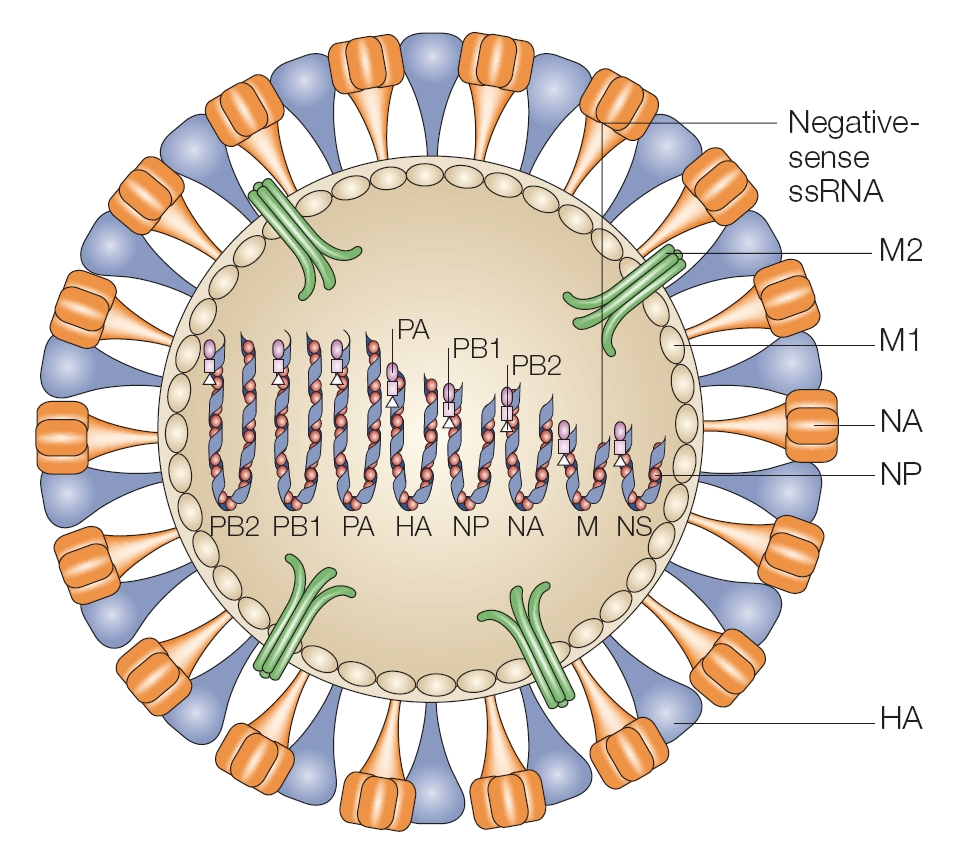
\includegraphics[width=.5\columnwidth]{./fig/influenza/flu_genome.jpg}}
\caption[Structure of an influenza virus particle]{Structure of an influenza virus particle. Surface antigens HA and NA coat this surface and are involved in viral entry and exit into the host cell. The surface capsid is formed from matrix proteins M1 and M2. PB1, PB2, and PA form a polymerase complex assisting in viral replication in the infected cell.}
\label{fig:flu:genome}
\end{center}
\end{figure}

\section{Influenza Reassortment}
\label{flu:reassortment}

We characterized reassortment in avian influenza using persistent homology.
We first compiled an aligned dataset of 3,105 complete avian influenza genomes from the NIH Influenza Sequence Database.
These sequences span in time from 1956 to 2012. 
We collected samples from all influenza subtypes.
The majority of our sequences are of the H5 and H6 type, with a smaller proportion of H3, H7, and H9.
The distribution of collected HA types and years is shown in Figure~\ref{fig:flu:histograms}.

\begin{figure}
\centering
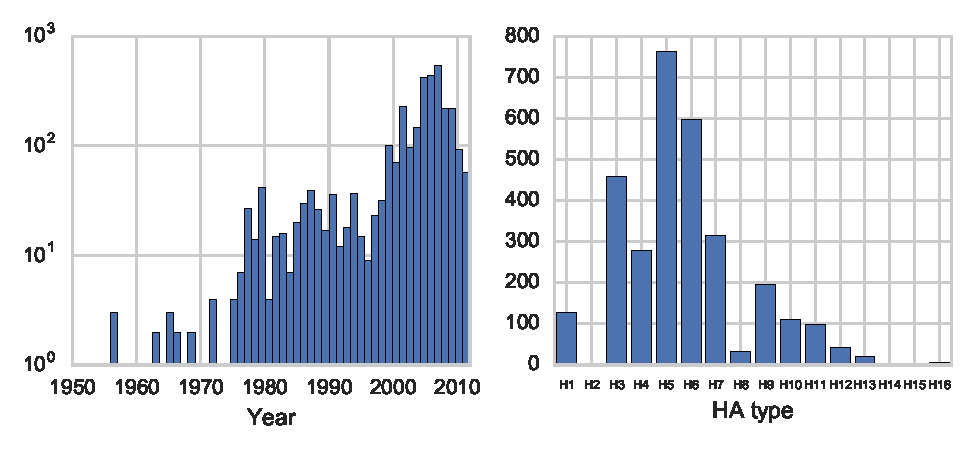
\includegraphics[]{fig/influenza/flu_histograms.pdf}
\caption[Influenza Dataset Statistics]{The avian influenza dataset analyzed in this chapter. Sequences spanned from 1950 to 2011, with the vast majority being collected after 2000. Most sequences were of HA type H5, with H6 and H3 following. Dataset was collected from the NCBI Influenza Virus Resource \cite{Bao:2008cq}}
\label{fig:flu:histograms}
\end{figure}

We first applied persistent homology to each genomic segment individually, as shown in Figure~\ref{fig:flu:segment_barcodes}.
Here we see very little higher homology, consistent with no intra-segmental recombination.
The presence of higher homology is likely due to back mutation, which is expected to be more common in viruses with high mutation rates and shorter genomes (i.e. the infinite sites model does not hold).
However, an analysis of the concatenated full genome reveals a complex topology, with a large number of homological invariants in one and two dimensions (Figure~\ref{fig:flu:concatenated_genome_barcode}.

These results show that persistent homology can detect pervasive reassortment in influenza.
One-dimensional $\ICR$ provides a lower-bound estimate of reassortment rate.
We calculate $\ICR < 1$ event per year for classic H1N1 swine and H3N2 human influenza, supported by previous phylogenetic estimates \cite{Lycett:2012fqa,Holmes:2005cia}.
In contrast, we calculate a high rate of 22.16 reassortments per year for avian influenza A.
This difference could be explained by the high diversity and frequent coinfection of avian viruses \cite{Lubeck:1979ws} and correlates with the high proportion of avian reassortants reported in previous studies \cite{Dugan:2008iba}.

\begin{figure}
\centering
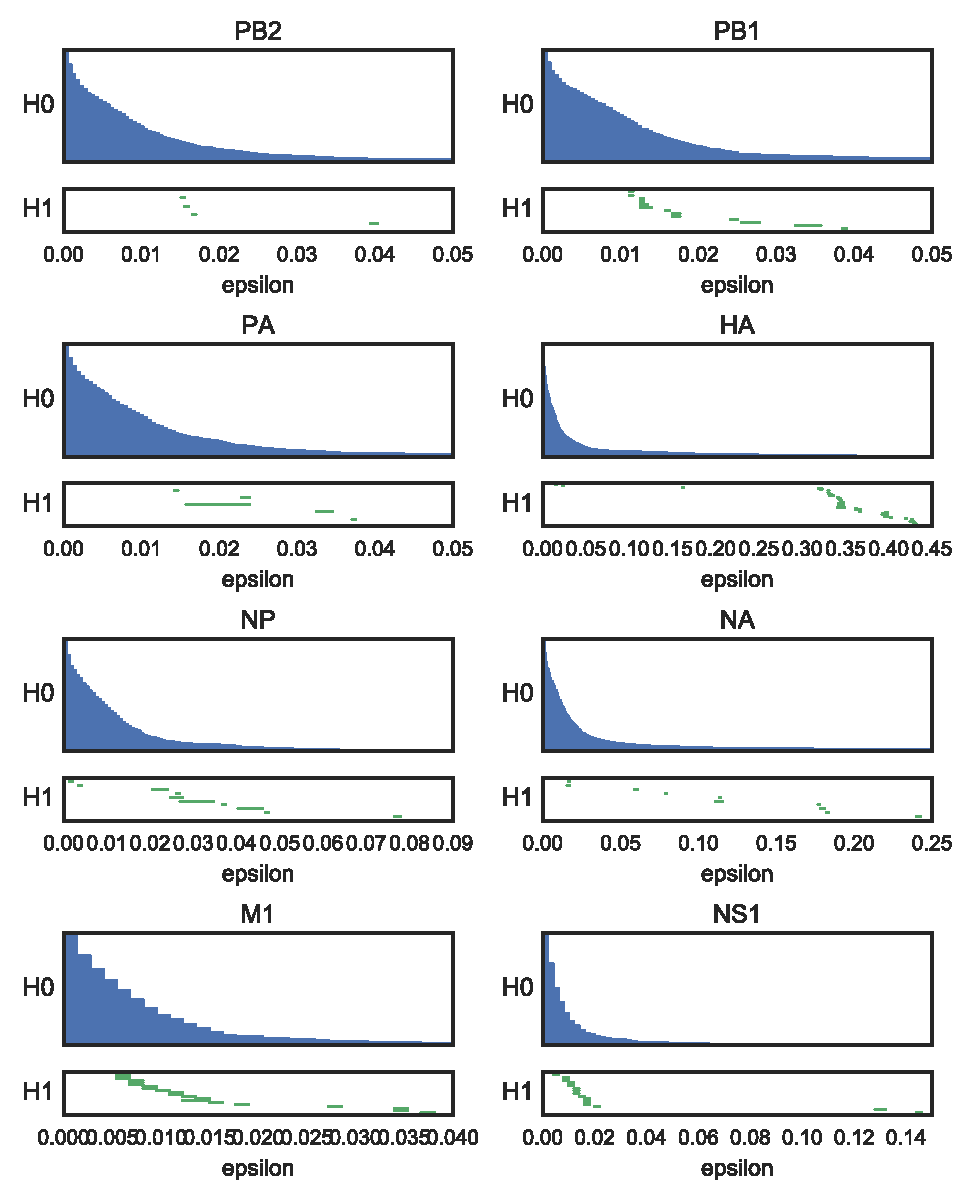
\includegraphics[]{fig/influenza/flu_segment_barcodes.pdf}
\caption[Influenza Genome Segment Barcodes]{Influenza Genome Segment Barcodes. Persistent homology computed on a per-segment basis reveals very little $H_1$ homology, indicating limited intrasegment reticulation.}
\label{fig:flu:segment_barcodes}
\end{figure}

\begin{figure}
\centering
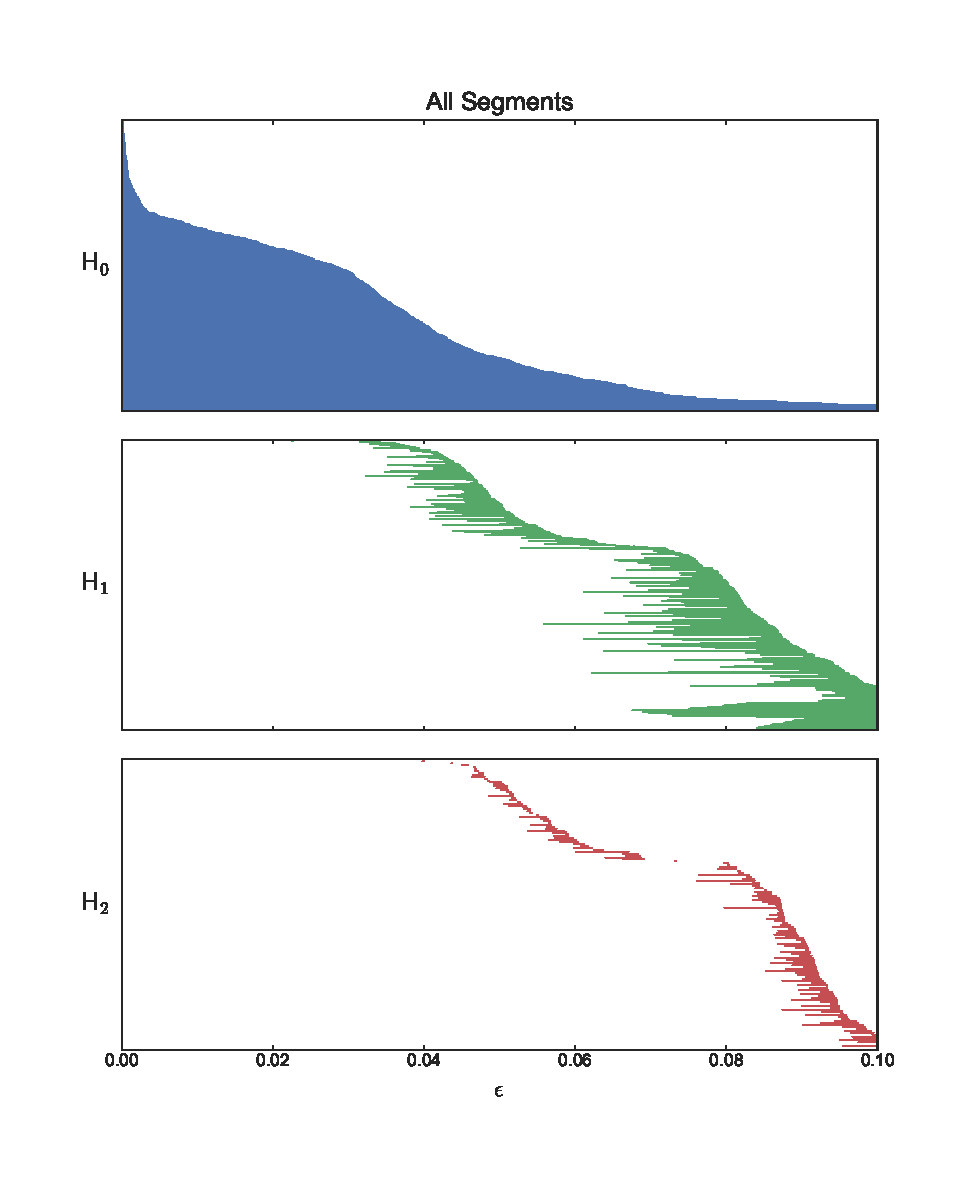
\includegraphics[]{fig/influenza/flu_concat_barcode.pdf}
\caption[Influenza Concatenated Genome Barcode]{Influenza Concatenated Genome Barcode. Persistent homology computed on the full concatenated genome reveals substantial $H_1$ and $H_2$ homology, indicating high levels of reticulate exchange.}
\label{fig:flu:concatenated_genome_barcode}
\end{figure}

We used mapper to visualize the relationships in our influenza dataset.
A series of mapper networks is shown in Figure~\ref{fig:flu:networks_by_subtype}.
The networks were generated using a Hamming metric and the first and second MDS components as a 2D lens.
In each subfigure we color the network by influenza subtype, for the top ten subtypes represented in the dataset.
We can see that the current classification of flu sequences by HA and NA type is a reasonable approach, as flu isolates of same subtype tend to cluster together tightly within the network.
H6N2 is the sole subtype to be represented by two clusters in the network.
When we examined the members of each H6N2 cluster, we found that both consisted of isolates spanning long time frames, suggesting that multiple stable lineages of H6N2, each carrying different internal segments, have persisted.

The Mapper representation offers further resolution into isolate relationships that can account for whole genomes.
We performed an MCL clustering of the network and considered how subtype-pure each cluster was.
\kje{TODO: Make the figure and expand here. Explain alternate classification scheme.}

\begin{figure}
\centering
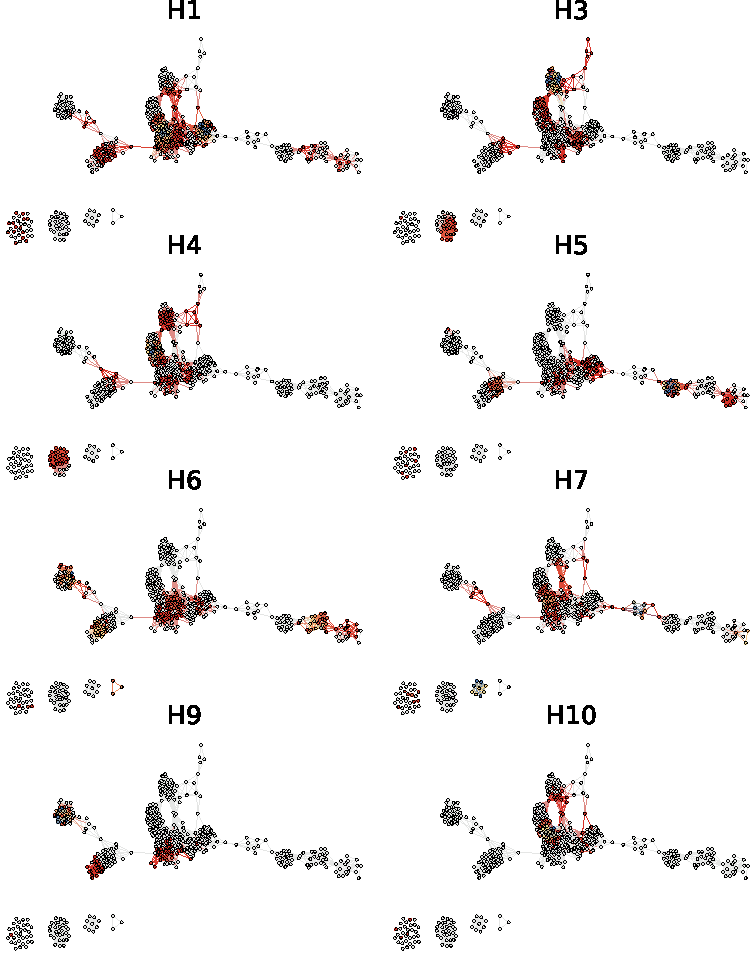
\includegraphics[width=\textwidth]{fig/influenza/flu_networks_by_subtype.pdf}
\caption[Influenza Networks By HA Subtype]{Influenza Networks By HA Subtype. The networks were generated using Ayasdi. [Parameters]}
\label{fig:flu:networks_by_subtype}
\end{figure}

\section{Nonrandom Association of Genome Segments}
\label{flu:nonrandom_reassortment}

We observed nonrandom association of flu segments.
Statistical inference on the loops corresponding to reassortments identified segments that tend to co-segregate with each other during reassortment.In particular, polymerases co-segregate, while genes coding for envelope and capsid proteins show independent reassortment patterns.
Cosegregation of polymerases suggests that effective protein–protein interaction between the polymerase complex and the NP protein constrain reassortment. 

Although previous phylogenetic studies confirmed a high reassortment rate in avian influenza, none has identified a clear pattern of gene segment association \cite{Dugan:2008iba}.
To determine whether any segments cosegregate more than expected by chance, we considered all pairs of concatenated segments and estimated the number of reassortments using $b_{1}$.
We then ascertained the significance of observing a number of reassortments between each pair of segments given the total estimate of reassortments in the concatenated genome.
These patterns of cosegregation are represented in Figure~\ref{fig:flu:nonrandom_reassortment}, in which thicker edges indicate cosegregation, as measured by a lower level of homology between segment pairs.
% \kje{TODO: Put statistics in a table}
Analysis of avian influenza reveals a statistically significant configuration of four cosegregating segments: polymerase basic 2 (PB2), polymerase basic 1 (PB1), polymerase acidic (PA), and nucleoprotein (NP).
Interestingly, this pattern mimics previous in vitro results that suggest that effective protein-–protein interaction between the polymerase complex and the NP protein constrain reassortment \cite{Lubeck:1979ws}.

\begin{figure}
\begin{center}
\centerline{
\includegraphics[width=\columnwidth]{./fig/influenza/flu_reassortment_correlations.pdf}}
\caption[Influenza Nonrandom Reassortment]{Influenza Nonrandom Reassortment}
\label{fig:flu:nonrandom_reassortment}
\end{center}
\end{figure}

\section{Multiscale Flu Reassortment}
\label{flu:multiscale_reassortment}

We computed persistent homology on the avian influenza sequences across the seven major HA subtypes.
The persistence diagram is shown in Figure \ref{fig:flu:scatterplot}, along with density estimates for the birth and death distributions.
Both birth and death times appear strongly bimodal, unlike in the coalescent simulations, which were strictly unimodal.
This suggests two distinct scales of topological structure.
Using the representative cycles output by Dionysus on a subset of this data, we classified features as intrasubtype (involving one HA subtype) and intersubtype (involving multiple HA subtypes).
The $H_1$ barcode diagram for this data is shown in the Figure \ref{fig:flu:scatterplot} inset.
Intrasubtype features, in blue, occur at an earlier filtration scale than intersubtype features, in green.
The multiscale topological approach of persistent homology can distinguish biological events occuring at different genetic scales.

We isolated the two peaks and estimated two recombination rates: an intrasubtype $\rho_{1}=9.68$, and an intersubtype $\rho_{2}=21.43$.
We conclude that intersubtype recombination occurs at a rate over twice that of intrasubtype recombination, however a genetic barrier exists that maintains distinct subtype populations.
The nature of this barrier warrants further study.
This illustrates a real world example in which multiscale topological structure can be captured by persistent homology and given biological interpretation.

\begin{figure}
\centering
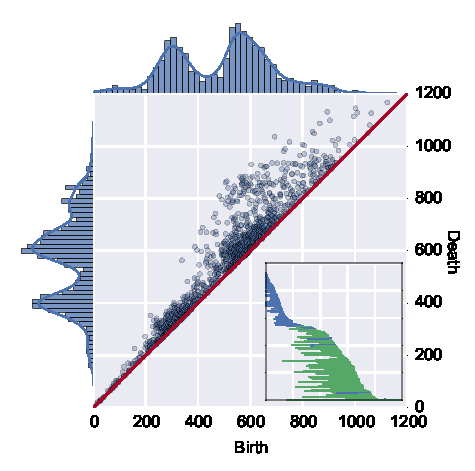
\includegraphics[width=\columnwidth]{./fig/influenza/flu_scatterplot.pdf}
\caption[$H_1$ persistence diagram computed from an avian influenza dataset.]{The $H_1$ persistence diagram computed from an avian influenza dataset. On the top and left are plotted the marginal distributions of birth and death times, along with a density estimate for each distribution. The bimodality indicates two scales of topological structure. Inset: The barcode diagram for a subset of this data. Blue bars have representative cycles involving only one subtype, green bars have cycles involving multiple subtypes.}
\label{fig:flu:scatterplot}
\end{figure}

\section{Conclusions}
\label{flu:conclusions}

In this chapter we analyzed reassortment patterns in influenza.
The segmented nature of the influenza genome, and the large amount of collected genome information, make influenza ideal for the application of our topological methods.
Reassortment occurs when a single cell is coinfected by multiple strains of the virus, and can lead to the emergence of novel pandemics.
Current methods of classifying influenza, based solely on HA and NA subtype, fail to account for information in the internal segments and have no consistent methodology for dealing with reassortments.
We have applied methods from TDA to characterize both the scale and frequency of reassortment in influenza, estimating both reassortment rates and cosegregation patterns.
Using Mapper, we determined classifications of viruses based on whole genome information that provide a higher resolution picture into extant circulating strains.
Further, from the persistence diagram we identified a bimodal structure of $H_1$ invariants, which suggests a genetic barrier maintaining subtype diversity.

% Pathogenic Bacteria
% From Warsaw conference paper
%!TEX root = ../../thesis.tex
\chapter{Reticulate Evolution in Pathogenic Bacteria}
\label{ch:pathogens}

\section{Introduction}
\label{pathogens:introduction}

Pathogenic bacteria can lead to severe infection and mortality and present an enormous burden on human populations and public health systems.
One of the achievements of twentieth century medicine was the development of a wide range of antibiotic drugs to control and contain the spread of pathogenic bacteria, leading to vastly increased life expectancies and global economic development.
However, rapidly rising levels of multidrug antibiotic resistance in several common pathogens, including \emph{Escherichia coli}, \emph{Klebsiella pneumoniae}, \emph{Staphylococcus aureus}, and \emph{Neisseria gonorrhoeae}, is recognized as a pressing global issue with near-term consequences \cite{Neu:1992gk,Thomas:2005hp,WHO:2014wa}.
The threat of a post-antibiotic 21st century is serious, and new methods to characterize and monitor the spread of resistance are urgently needed.

Antibiotic resistance can be acquired through point mutation or through horizontal transfer of resistance genes.
Horizontal exchange occurs when a donor bacteria transmits foreign DNA into a genetically distinct bacteria strain.
As discussed in Chapter~\ref{ch:background}, three mechanisms of horizontal transfer have been identified, depending on the route by which foreign DNA is acquired \cite{Ochman:2000dr}.
Foreign DNA can be acquired via uptake from an external environment (transformation), via viral-mediated processes (transduction), or via direct cell-to-cell contact between bacterial strains (conjugation).
Resistance genes can be transferred between strains of the same species, or can be acquired from different species in the same environment.
While the former is generally more common, an example of the latter is the phage-mediated acquisition of Shiga toxin in \emph{E. coli} in Germany in 2011 \cite{Rohde:2011ju}.
Elements of the bacterial genome that show evidence of foreign origin are called genomic islands, and are of particular concern when associated with phenotypic effects such as virulence or antibiotic resistance.

In this chapter we explore topics relating to horizontal gene transfer in bacteria and the emergence of antibiotic resistance in pathogenic strains.
We show that TDA can not only quantify gene transfer events, but also characterize the scale of gene transfer.
The scale of recombination can be measured from the distribution of birth times of the $H_1$ invariants in the barcode diagram.
It has been shown that recombination rates decrease with increasing sequence divergence \cite{Fraser:2007ep}.
We characterize the rate and scale of intraspecies recombination in several pathogenic bacteria of public health concern.
We select a set of pathogenic bacteria that are of public health interest based on a recently released World Health Organization (WHO) report on antimicrobial resistance \cite{WHO:2014wa}.
Using persistent homology, we characterize the rate and scale of recombination in the core genome using multilocus sequence data.
To extend our characterization to the whole genome, we use protein family annotations as a proxy for sequence composition.
This allows us to compute a similarity matrix between strains.
Comparing persistence diagrams gives us information about the relative scales of gene transfer at arbitrary loci.
The species selected for study and the sample sizes in each analysis are specified in Table~\ref{table:samplesizes}.
Next, we explore the spread of antibiotic resistance genes in \emph{S. aureus} using Mapper, an algorithm for partial clustering and visualization of high dimensional data \cite{Singh:2007ve}.
We identify two major populations of \emph{S. aureus}, and observe one cluster with strong enrichment for the antibiotic resistance gene \emph{mecA}.
Importantly, resistance appears to be increasingly spreading in the second population.
Finally, we consider the risk of lateral transfer of resistance genes from the human microbiome into an antibiotic sensitive strain, using $\beta$-Lactam resistance as an example.
In this environment, benign bacterial strains can harbor known resistance genes.
We use a network analysis to visualize the spread of antibiotic resistance gene $\emph{mecA}$ into nonnative phyla.
Each individual has a unique microbiome, and we speculate that microbiome typing of this sort may useful in developing personalized antibiotic therapies.
These results suggest an important role for topological data mining of -omics scale data in clinical applications and personalized medicine.

\begin{table}
\centering
\caption[List of pathogenic bacteria selected for study]{Pathogenic bacteria selected for study and sample sizes in each analysis.}
\begin{tabularx}{\textwidth}{Xcc}
\toprule
Species & \hspace{10mm}MLST profiles\hspace{10mm} & PATRIC profiles \\
\midrule
\emph{Campylobacter jejuni}      & 7216  & 91 \\
\emph{Escherichia coli}          & 616   & 1621 \\
\emph{Enterococcus faecalis}     & 532   & 301 \\
\emph{Haemphilus influenzae}     & 1354  & 22 \\
\emph{Helicobacter pylori}       & 2759  & 366 \\
\emph{Klebsiella pneumoniae}     & 1579  & 161 \\
\emph{Neisseria spp.}            & 10802 & 234 \\
\emph{Pseudomonas aeruginosa}    & 1757  & 181 \\
\emph{Staphylococcus aureus}     & 2650  & 461 \\
\emph{Salmonella enterica}       & 1716  & 638 \\
\emph{Streptococcus pneumoniae}  & 9626  & 293 \\
\emph{Streptococcus pyogenes}    & 627   & 48 \\
\bottomrule
\end{tabularx}
\label{table:samplesizes}
\end{table}

\section{Evolutionary Scales of Recombination in the Core Genome}
\label{pathogens:mlst}
%
Multilocus sequence typing (MLST) data was used to examine scales of recombination in the core bacterial genome.
MLST is a method of rapidly assigning a sequence profile to a sample bacterial strain.
For each species, a predetermined set of loci in a small number of housekeeping genes are selected as representative of the core genome of the species.
At each loci, a set of sequence types are defined by using a similarity-based clustering.
As new strains are sequenced, they are annotated with a profile corresponding to the type at each locus.
If a sample has a previously unseen type at a given locus, it is appended to the list of types at that locus.
Large online databases have curated MLST data from labs around the world; significant pathogens can have several thousand typed strains (over 10,000 in the case of \emph{Neisseria spp.}).
Because different species will be typed at different loci, examining direct interspecies genetic exchange with this data is unfeasible, however MLST provides a large quantity of data with which to examine intraspecies exchange in the core genome.
Finally, because the selected loci are primarily housekeeping genes, this type of recombination analysis will tell you only about genetic exchange in the core genome.
Mobile genetic elements may have a separate rates of exchange.

We investigate genetic exchange in the twelve pathogens using MLST data from PubMLST \cite{Jolley:2010gf}.
For each strain, a pseudogenome can be constructed by concatenating the typed sequence at each locus.
Using a Hamming metric, we construct a pairwise distance matrix between strains and compute persistent homology on the resulting metric space.
Because of the large number of sample strains, we employ a Lazy Witness complex with 250 landmark points and $\nu=0$ \cite{deSilva:2004tg}.
The computation is performed using javaplex \cite{Tausz:2011}.
An example of our output is shown in Figure~\ref{fig:pathogen_barcodes}, where we plot the $H_1$ barcode diagrams for \emph{K. pneumoniae} and \emph{S. enterica}.
The two species have distinct recombination profiles, characterized by the range of recombinations: \emph{K. pneumoniae} recombines at only an early short-lived scale, while \emph{S. enterica} recombines both at the short-lived scale and a longer-lived scale.
These multiple scales are reflective of population structure at the subspecies level: in \emph{S. enterica}, there are seven defined subspecies, and experimental studies have shown high levels of reticulation both within and between subspecies groups \cite{Brown:2003id}.
We repeat this analysis for each species, and plot the results as a persistence diagram in Figure~\ref{fig:pathogen_persistence_diagram}.
Among the bulk of pathogens there appears to be three major scales of recombination, a short-lived scale at intermediate distances, a longer-lived scale at intermediate distances, and a short-lived scale at longer distances.
We recover a pronounced pattern of reticulation at very short distances unique to \emph{H. Pylori}, which is consistent with earlier measurements of an unusually small size of DNA imports, reported in \cite{Falush:2001cd}.

\begin{figure}
    \centering
    \subbottom[\emph{Klebsiella pneumoniae}]{
        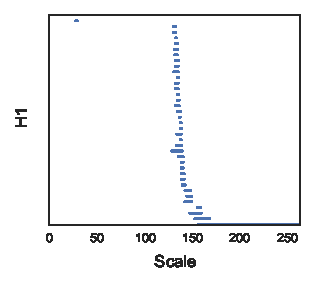
\includegraphics[width=.4\textwidth]{./fig/pathogens/kpneumoniae_barcode.pdf}}
    \subbottom[\emph{Salmonella enterica}]{
        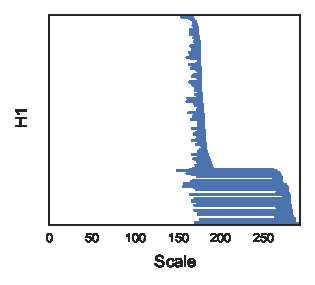
\includegraphics[width=.4\textwidth]{./fig/pathogens/senterica_barcode.pdf}}
    \caption[Core genome exchange in \emph{K. pneumoniae} and \emph{S. enterica}]{Barcode diagrams reflect different scales of core genomic exchange in \emph{K. pneumoniae} and \emph{S. enterica}. Differing scales can be attributed to different degrees of population substructure in the two species.}
    \label{fig:pathogen_barcodes}
\end{figure}

\begin{figure}
\centering
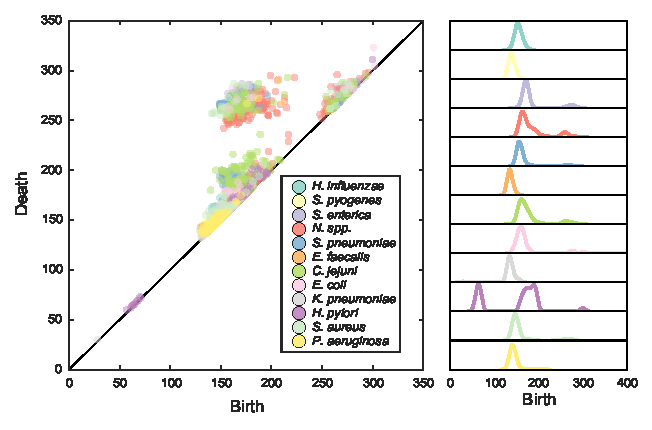
\includegraphics[width=\textwidth]{./fig/pathogens/pathogen_persistence_diagram.pdf}
\caption[$H_1$ persistence diagram for twelve pathogenic strains using MLST profile data]{The $H_1$ persistence diagram for the twelve pathogenic strains selected for this study using MLST profile data. There are three broad scales of recombination. To the right is the birth time distribution for each strain. \emph{H. pylori} has an earlier scale of recombination not present in the other species, corresponding to the atypically small size of DNA imports in the species \cite{Falush:2001cd}.}
\label{fig:pathogen_persistence_diagram}
\end{figure}

We define a relative rate of recombination by counting the total number of $H_1$ loops across the filtration and dividing by the number of samples for that species.
The results are shown in Figure~\ref{fig:pathogen_barchart}, where we observe that different species can have vastly different reticulation profiles.
For example, \emph{S. enterica} and \emph{E. coli} have the highest reticulation rates, consistent with earlier results which have shown a high proportion of defects in the \emph{mutS} mismatch-repair gene leading to relaxed genetic barriers to recombination \cite{Rayssiguier:1989gb,LeClerc:1996hx}.
The low measured reticulation rate in \emph{H. pylori} is a surprising outlier, as previous studies have shown that it lacks the mismatch repair pathways common in other bacteria, leading to higher than expected recombination rates \cite{Dorer:2011hx}.
\emph{H. pylori} has been reported to have very little clonal structure relative to other strains, which is reflected in the star-like phylogeny that has been proposed for the species \cite{Kalia:2004jx}
However, restriction-modification systems limiting uptake of foreign DNA have also been reported \cite{Dwivedi:2013bt}, suggesting that the \emph{H. pylori} core genome is relatively resistant to reticulation at wider genomic scales.
It is therefore plausible that the lower signal from persistent homology is due to systematic reduced sampling of particular lineages, suggesting that accounting for larger-scale population structure is important when making estimates of reticulation rates.

\begin{figure}
\centering
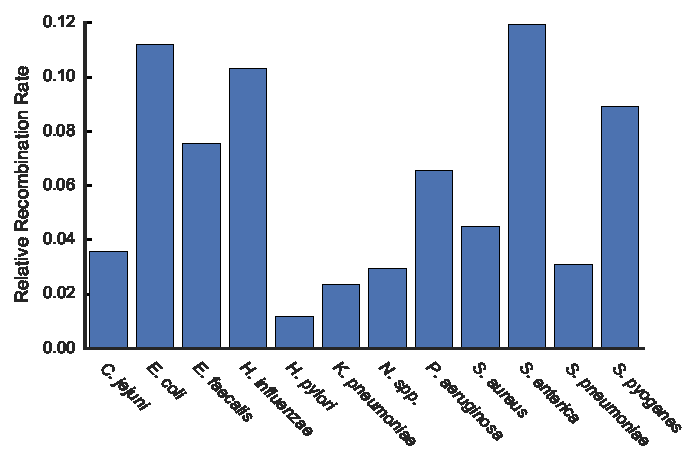
\includegraphics[width=\textwidth]{./fig/pathogens/pathogen_barchart.pdf}
\caption[Core genome reticulation patterns in pathogenic bacteria from MLST profiles]{Relative recombination rates computed by persistent homology from MLST profile data.}
\label{fig:pathogen_barchart}
\end{figure}

\section{Protein Families as a Proxy for Genome Wide Reticulation}
\label{pathogens:patric_analysis}

Protein family annotations cluster proteins into sets of isofunctional homologs, i.e., clusters of proteins with both similar sequence composition and similar function.
A particular strain is represented as a binary vector indicating the presence or absence of a given protein family.
Correlations between strains can reveal genome-wide patterns of genetic exchange, unlike the MLST data which can only provide evidence of exchange in the core genome.
We use the FigFam protein annotations in the Pathosystems Resource Institute Center (PATRIC) database because of the breadth of pathogenic strain coverage and depth of genomic annotations \cite{Wattam:2013jy}.
The FigFam annotation scheme consists of over 100,000 protein families curated from over 950,000 unique proteins \cite{Meyer:2009iq}.

For each strain we compute a transformation into FigFam space.
We transform into this space because the frequency of genome rearrangements and differences in mobile genetic elements makes whole genome alignments unreliable, even for strains within the same species.
As justification for performing this step, it has been shown experimentally that recombination rates decrease with increasing genetic distance \cite{Fraser:2007ep}.
After transforming, we construct a strain-strain correlation matrix and compute the persistent homology in this space.
In Figure~\ref{fig:figfam_persistence_diagram} we show the persistence diagram relating the structure and scale between different species.
We find that different species have a much more diverse topological structure in this space than in MLST space, and a wide variety of recombination scales.
The large scales of exchange in \emph{H. influenzae} suggest it can regularly acquire novel genetic material from distantly related strains.
% TODO: why? this is correlation across genome - very mosaic?

\begin{figure}
\centering
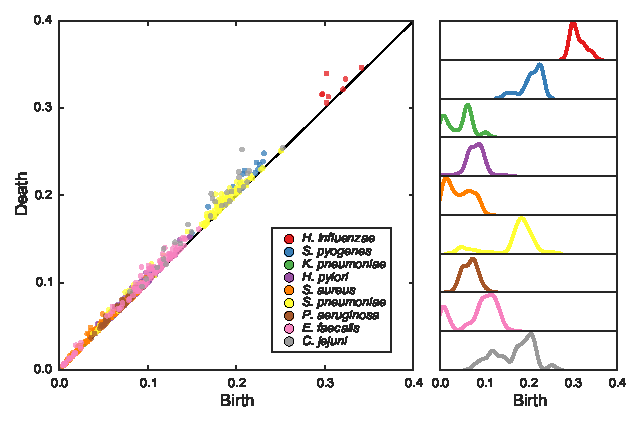
\includegraphics[width=\textwidth]{./fig/pathogens/figfam_persistent_diagram.pdf}
\caption[Genome-wide reticulation patterns in pathogenic bacteria from protein annotations]{Persistence diagram for a subset of pathogenic bacteria, computed using the FigFam annotations compiled from PATRIC. Compared to the MLST persistence diagrams, the Figfam diagrams have a more diverse scale of topological structure.}
\label{fig:figfam_persistence_diagram}
\end{figure}

\section{Antibiotic Resistance in \emph{Staphylococcus aureus}}
\label{sec:staph_aureus}
%
\emph{S. aureus} is a gram positive bacteria commonly found in the nostrils and upper respiratory tract.
Certain strains can cause severe infection in high-risk populations, particularly in the hospital setting.
The emergence of antibiotic resistant \emph{S. aureus} is therefore of significant clinical concern.
Methicillin resistant \emph{S. aureus} (MRSA) strains are resistant to $\beta$-lactam antibiotics including penicillin and cephalosporin.
Resistance is conferred by the gene \emph{mecA}, an element of the Staphylococcal cassette chromosome mec (\emph{SCCmec}).
\emph{mecA} codes for a dysfunctional penicillin-binding protein 2a (PBP2a), which inhibits $\beta$-lactam antibiotic binding, the primary mechanism of action \cite{Jensen:2009fu}.
Of substantial clinical importance are methods for characterizing the spread of MRSA within the \emph{S. aureus} population.

To address this question, we use the FigFam annotations in PATRIC, as described in the previous section.
PATRIC contains genomic annotations for 461 strains of \emph{S. aureus}, collectively spanning 3,578 protein families.
We perform a clustering analysis using the Mapper algorithm as implemented in Ayasdi Iris \cite{AyasdiIris:2015}.
Principal and second metric singular value decomposition are used as filter functions, with a 4x gain and an equalized resolution of 30.
This results in a graph structure with two large clusters, with a smaller bridge connecting the two, as shown in Figure~\ref{fig:saureus_figfam_network}.
The two clusters are consistent with previous phylogenetic studies using multilocus sequence data to identify two major population groups \cite{Cooper:2006dp}.

Of the 461 \emph{S. aureus} strains in PATRIC, 142 carry the \emph{mecA} gene.
When we color nodes in the network based on an enrichment for the presence of \emph{mecA}, we observe a much stronger enrichment in one of the two clusters.
This suggests that $\beta$-lactam resistance has already begun to dominate in that clade, likely due to selective pressures.
More strikingly, we observe that while \emph{mecA} enrichment is not as strong in the second cluster, there is a distinct path of enrichment emanating along the connecting bridge between the two clusters and into the less enriched cluster.
This suggests the hypothesis that antibiotic resistance has spread from the first cluster into the second cluster via strains intermediate to the two, and will likely continue to be selected for in the second cluster.

\begin{figure}[t]
\centering
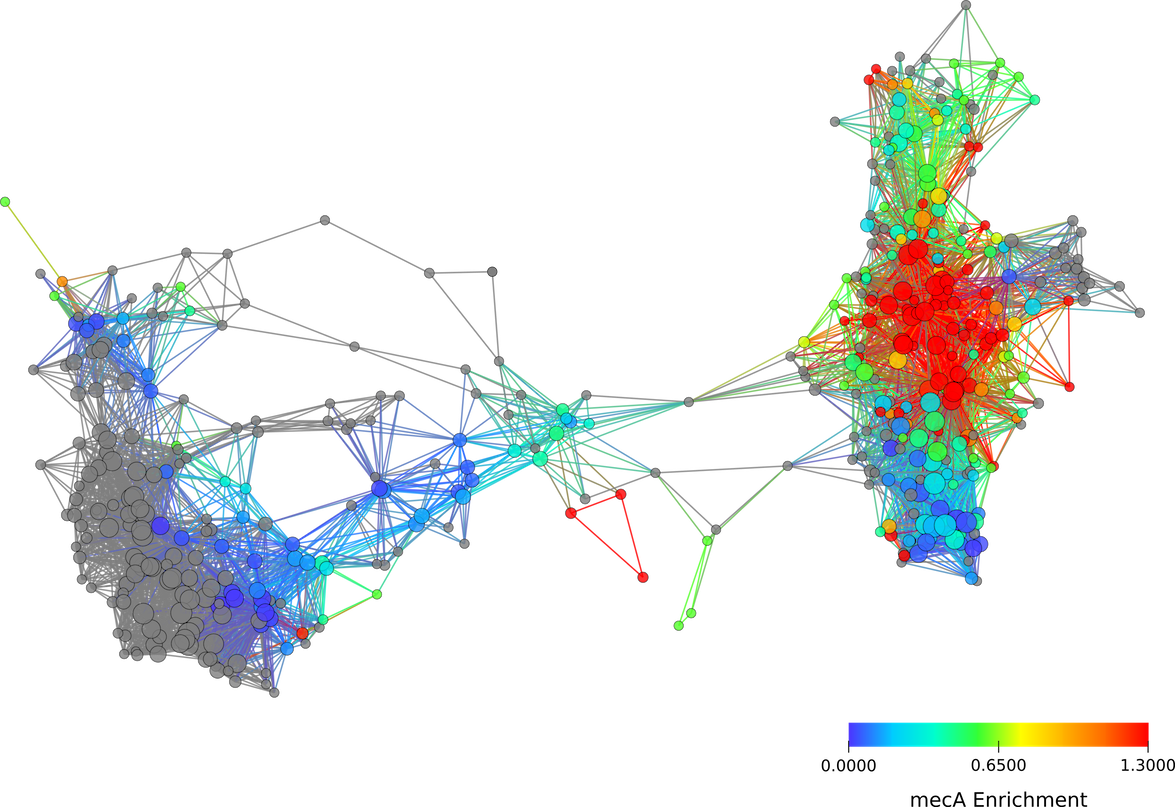
\includegraphics[width=\textwidth]{./fig/pathogens/saureus_figfam_network.png}
\caption[FigFam similarity network of \emph{S. aureus}]{The FigFam similarity network of \emph{S. aureus} constructed using Mapper as implemented in Ayasdi Iris \cite{AyasdiIris:2015}. We use a Hamming metric and Primary and Secondary Metric SVD filters (res: 30, gain 4x, equalize). Node color is based on strain enrichment for \emph{mecA}, the gene conferring $\beta$-Lactam resistance. Two distinct clades of \emph{S. aureus} are visible, one of which has already been compromised for resistance. Of important clinical significance is the growing enrichment for \emph{mecA} in the second clade.}
\label{fig:saureus_figfam_network}
\end{figure}

\section{Microbiome as a Reservoir of Antibiotic Resistance Genes}
\label{pathogens:microbiome}

While antibiotic resistance can be acquired through gene exchange between strains of the same species, it is also possible for gene exchange to occur between distantly related species.
It has been recognized that an individual's microbiome, the set of microorganisms that exist symbiotically within a human host, can act as a reservoir of antimicrobial resistance genes \cite{Sommer:2010uh,Penders:2013wt}.
It is of substantial clinical interest to characterize to what extent an individual's microbiome may pose a risk for a pathogenic bacteria acquiring a resistance gene through lateral transfer.

To address this question, we use data from the Human Microbiome Project (HMP), a major research initiative performing metagenomic characterization of hundreds of healthy human microbiome samples \cite{Consortium:2012bm}.
The HMP has defined a set of reference strains that have been observed in the human microbiome.
We collect FigFam annotations from PATRIC for the reference strain list in the gastrointestinal tract.
We focus on the gastrointestinal tract because it is an isolated environment and likely to undergo higher rates of exchange than other anatomic regions.
Of the 717 reference strains, 321 had FigFam annotations.
We computed a similarity matrix as in previous sections, using correlation as distance.
The resulting network is shown in Figure~\ref{fig:microbiome_network}, where strains are colored by phyla-level classifications.
While largely recapitulating phylogeny, the network depicts interesting correlations between phyla, such as the loop between Firmicutes, Bacteroides, and Proteobacteria.

Next, we searched for genomic annotations relating to $\beta$-lactam resistance.
10 strains in the reference set had matching annotations, and we highlight those strains in the network with green diamonds.
We observe resistance mostly concentrated in the Firmicutes, of which \emph{S. aureus} is a member, however there is a strain of Proteobacteria that has acquired the resistance gene.
Transfer of beta-lactam resistance into the Proteobacteria is clinically worrisome.
Pathogenic Proteobacteria include \emph{S. enterica}, \emph{V. cholerae}, and \emph{H. pylori}, and emergence of $\beta$-lactam resistance will severely impact antibiotic drug therapies.

The species composition of each individual's microbiome can differ substantially due to a wide variety of poorly understood factors \cite{Consortium:2012bm}.
In this case, an individuals personal microbiome network will differ from the network we show in Figure~\ref{fig:microbiome_network}, which was constructed from the set of \emph{all} strains that have been reported across studies of multiple individuals.
The relative risk for acquiring self-induced resistance will therefore vary from person to person and by the infectious strain acquired.
However, a network analysis of this type will give clues as to possible routes by which antibiotic resistance may be acquired.
In the clinical setting, this could assist in developing personalized antibiotic treatment regimens.
We propose a more thorough expansion of this work, examining the full range of antibiotic resistance genes in order to quantify microbiome risk factors for treatment failure.
We foresee an era of genomically informed infectious disease management in the clinical setting, based on an understanding of a patient's personal microbiome profile.

\begin{figure}[t]
\centering
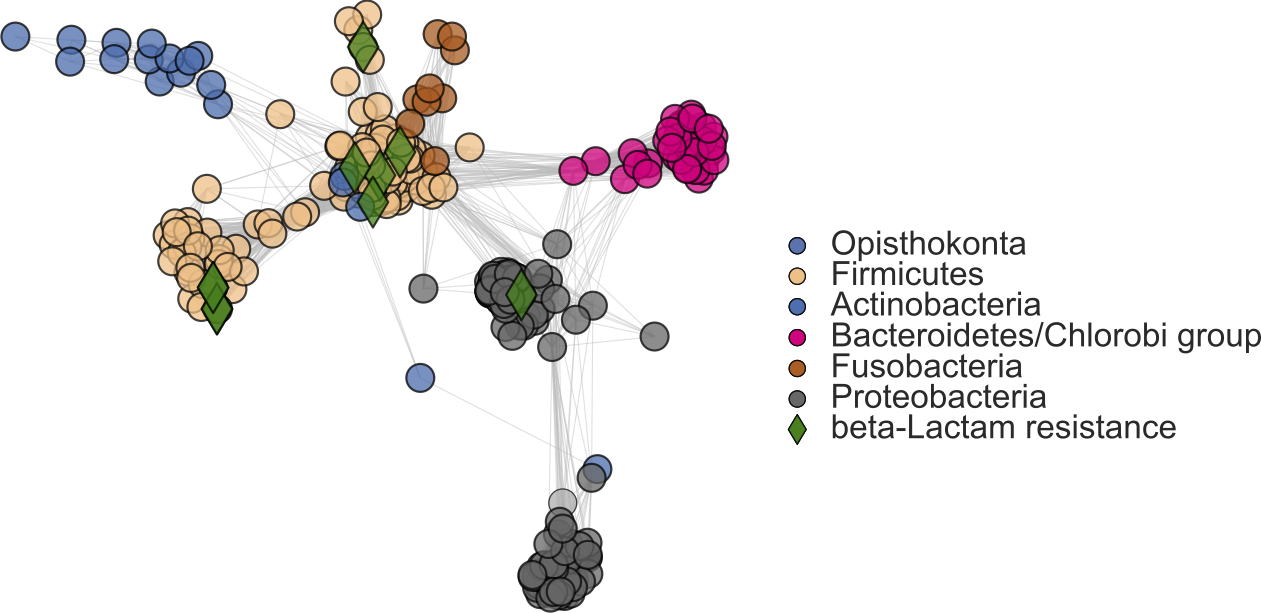
\includegraphics[width=\textwidth]{./fig/pathogens/microbiome_network.pdf}
\caption[FigFam similarity network of the gastrointestinal tract]{The FigFam similarity network of gastrointestinal tract reference strains identified in the Human Microbiome Project. The green diamond identifies the strains carrying resistance to $\beta$-Lactam antibiotics.}
\label{fig:microbiome_network}
\end{figure}

\section{Conclusions}

In this chapter we have used some ideas from topological data analysis to bear on problems in pathogenic microbial genetics.
First, we used persistent homology to evaluate recombination rates in the core genome using MLST profile data.
We showed that different pathogens have different recombination rates.
We expanded this to gene transfer across the whole genome by using protein family annotations in the PATRIC database.
We found different scales of recombination in different pathogens.
Second, we explored the spread of MRSA in \emph{S. aureus} populations using topological methods.
We noted increasing resistance in a previously isolated population.
Finally, we studied the emergence of $\beta$-lactam resistance in the microbiome, and proposed methods by which personal risk could be assessed by microbiome typing.
These results point to a role for graph mining and topological data mining in health and personalized medicine.

% Prokaryote Reticulate Evolution - Tree of Life
% Mostly from COGs, some from other papers.
% Run PH, Run Ayasdi. Make some basic statements.
% %!TEX root = ../../thesis.tex
\chapter{Prokaryote Reticulate Evolution - Tree of Life}
\label{ch:prokaryotes}

In this chapter we examine evolutionary relationships across the prokaryotic domain.
As input data, we use the Cluster of Orthologous Genes (COG) database at NCBI \cite{Galperin:2014ua}.
Using a combination of topological tools, we present a construction meant to extend the tree of life paradigm.

\section{Introduction}

In this chapter, we examine evolutionary relationships across the prokaryotic domain.

First, we use persistent homology to characterize reticulation.
Second, we use mapper to visualize evolutionary relationships.

\section{Materials and Methods}

As input data, we use the Cluster of Orthologous Genes (COG) database from NCBI \cite{Galperin:2014ua}

\section{Results}

To visualize relationships, we use the Mapper algorithm, as implemented in Ayasdi Iris.

\section{Conclusion}

In this chapter, we have examined evolutionary relationships across the prokaryotic domain.